\chapter{Testbenches} \label{ch:Testbench}
\chapterquote{Desire for nothing except desirelessness. Hope for nothing except to rise above all hopes. Want nothing and you will have everything.}{Meher Baba}

\graphicspath{{Chapters/Testbench/Figures/}}
\lstinputpath{Codes-VHDL/Chapter-Testbenches/VHDLCodes} %path is defined in mypreamble


%\section{Introduction}
In this chapter, UART communication is discussed for NIOS design. Values of Sin(x) is generated using NIOS and the data is  received by computer using UART cable. Since, onchip memory is smaller for storing these values, therefore external memory i.e. SDRAM is used. Further, the received data is stored in a file using `Tera Term' software; finally live-plotting of data is performed using Python.  

In this chapter, we will learn following topics, 
\begin{enumerate}
	\item UART interface,
	\item Receiving the data on computer using UART communication,
	\item SDRAM interface,
	\item Saving data generated by NIOS desgin to a file using `Tera Term',
	\item Updating a existing QSys design and corresponding VHDL and NIOS design,
	\item Live-plotting of data using Python. 
\end{enumerate}

\section{UART interface}
First, create a empty project with name `UartComm' (see Section \ref{sec:new_project}). Next, open the QSys from Tools$\rightarrow$Qsys. Add `Nios Processor', `On-chip RAM (with 20k total-memory-size), `JTAG UART' and `UART (RS-232 Serial Port)' (\textbf{all with default settings}). Note that, Baud rate for UART is set to `115200' (see Fig. \ref{fig:uart_settings}), which will be used while getting the data on computer. Lastly, connect these items as shown in Fig. \ref{fig:uart_qsys_conn}; save it as `Uart\_Qsys.qsys' and finally generate the Qsys system and close the Qsys. Please see Section \ref{sec:CreateGenerateQsys}, if you have problem in generating the QSys system.

\begin{figure}[!h]
	\centering
	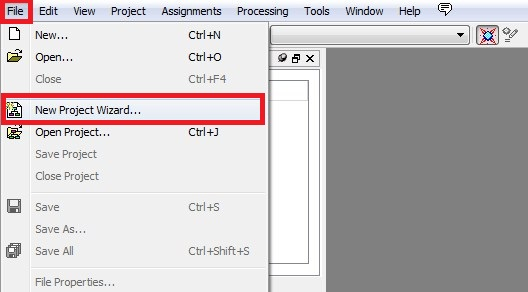
\includegraphics[scale=0.7]{1}
	\caption{UART settings}
	\label{fig:uart_settings}
\end{figure}
 
\begin{figure}[!h]
	\centering
	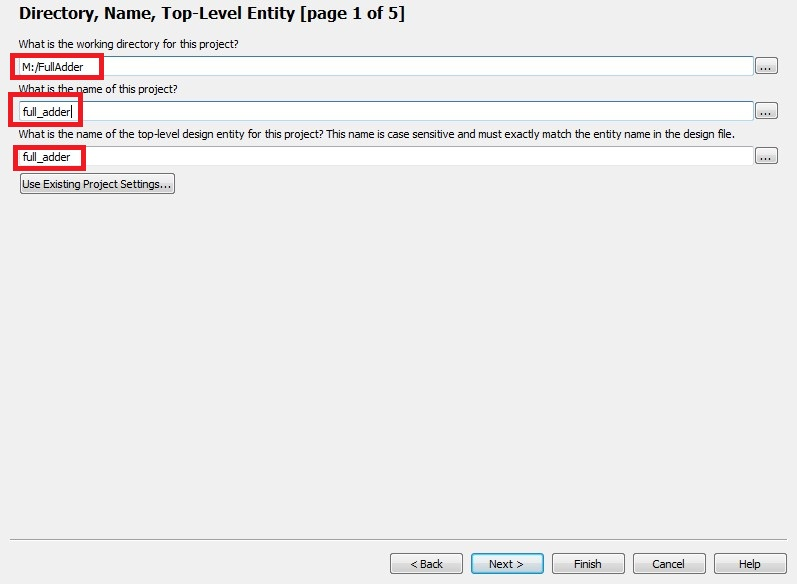
\includegraphics[scale=0.65]{2}
	\caption{Qsys connections}
	\label{fig:uart_qsys_conn}
\end{figure}

Now, add the file `Uart\_Qsys.qip' to the VHDL project. Next, create a new `Block diagram (.bdf) file and import the Qsys design to it and assign correct pin numbers to it, as shown in Fig. \ref{fig:uart_top}. Save it as `Uart\_top.bdf' and set it as `top  level entity'. Lastly, import the pin assignment file and compile the design. Finally, load the design on FPGA board. 

\begin{figure}[!h]
	\centering
	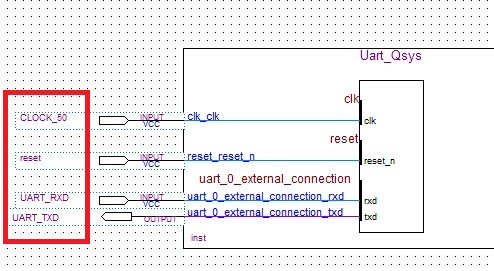
\includegraphics[scale=0.65]{3}
	\caption{Top level entity `Uart\_top.bdf'}
	\label{fig:uart_top}
\end{figure}

\section{NIOS design}
In Chapter \ref{ch:NiosOverview}, we created the `BSP' and `application' file separately for NIOS design. In this chapter, we will use the template provided with NIOS to create the design. For this, open the NIOS software and go to `Files$\rightarrow$New$\rightarrow$NIOS II Application and BSP from Template'. Next, Select the `UART\_Qsys.sopcinfo' file and `Hello World' template and provide the desired name to project e.g. UART\_comm\_app, as shown in Fig , and click `next'. In this window, enter the desired name for BSP file in the `Project name' column e.g. `UART\_comm\_bsp'; and click on Finish.  

\begin{figure}[!h]
	\centering
	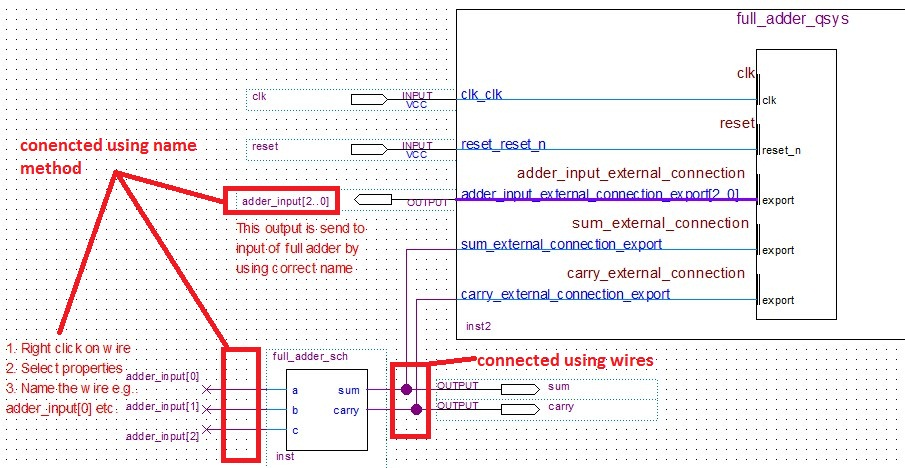
\includegraphics[scale=0.65]{4}
	\caption{Create NIOS project from template}
	\label{fig:nios_name_uart}
\end{figure}

\section{Communication through UART}
To received the data on computer, we need some software like Putty or Tera Term. In this tutorial, we are using `Tera Term software, which can be downloaded freely. Also, we need to change the UART communication settings; so that, we can get messages through UART interface (instead of JTAG-UART)  as shown next. 

Right click on `UART\_comm\_bsp' and go to `NIOS II$\rightarrow$BSP editor'; and select UART\_115200 for various communication as shown in Fig \ref{fig:nios_uart_settings}; and finally click on generate and then click on exit. Now, all the 	`printf' statements will be send to computer via UART port (instead of Jtag-uart). We can change it to JTAG-UART again, by changing UART\_115200 to JTAG-UART again. Note that, when we modify the BSP using BSP-editor, then we need to generate the system again.

\begin{figure}[!h]
	\centering
	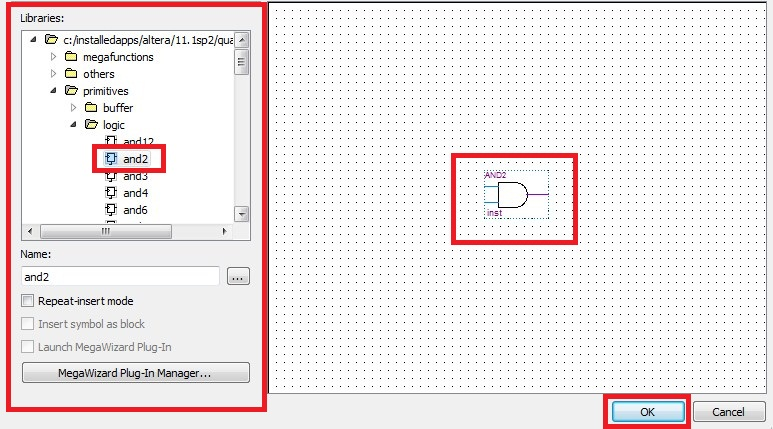
\includegraphics[scale=0.65]{5}
	\caption{UART communication settings in NIOS}
	\label{fig:nios_uart_settings}
\end{figure}

Now, open the Tera Term and select the `Serial' as shown in Fig. \ref{fig:teraTerm}. Then go to `Setup$\rightarrow$Serial Port...' and select the correct baud rate i.e. 115200 and click OK, as shown in Fig. \ref{fig:baudRateteraTerm}. 

\begin{figure}[!h]
	\centering
	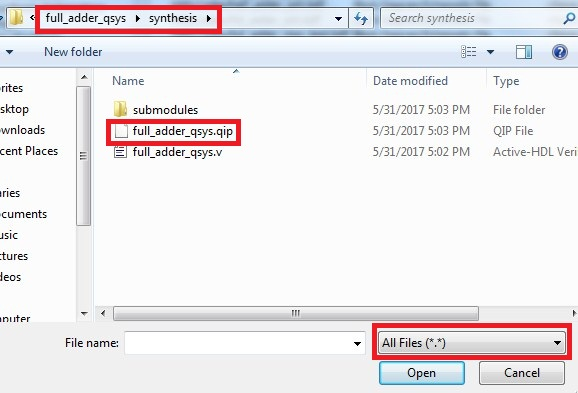
\includegraphics[scale=0.65]{6}
	\caption{Serial communication in Tera Term}
	\label{fig:teraTerm}
\end{figure}

\begin{figure}[!h]
	\centering
	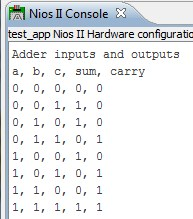
\includegraphics[scale=0.65]{7}
	\caption{Select correct baud rate}
	\label{fig:baudRateteraTerm}
\end{figure}

Finally, right click on `UART\_comm\_app' in NIOS and go to `Run As$\rightarrow$3 NIOS 2 Hardware'. Now, we can see the output on the Tera Term terminal, as shown in Fig. \ref{fig:helloTera}. 

\begin{figure}[!h]
	\centering
	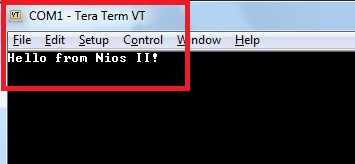
\includegraphics[scale=0.65]{8}
	\caption{`Hello from NIOS II!' on Tera Term}
	\label{fig:helloTera}
\end{figure}

\section{SDRAM Interface}
Our next aim is to generate the Sine waves using NIOS and then plot the waveforms using python. If we write the C-code in current design, then our system will report the memory issue as onchip memory is too small; therefore we need to use external memory. In this section, first, we will update the Qsys design with SDRAM interface, then we will update the Quartus design and finally add the C-code to generate the Sine waves. 

\subsection{Modify QSys}
First, Open the UART\_Qsys.qsys file in QSys software. Now, add SDRAM controller with default settings,  as shown in Fig. \ref{fig:sdram_con}. Next, connect all the ports of SDRMA as shown in Fig. \ref{fig:sdram_connections}. Then, double click the `nios2\_qsys\_0' and select `SDRAM' as reset and exception vector memory, as shown in Fig. \ref{fig:sdram_vector_memory}. 

\begin{figure}[!h]
	\centering
	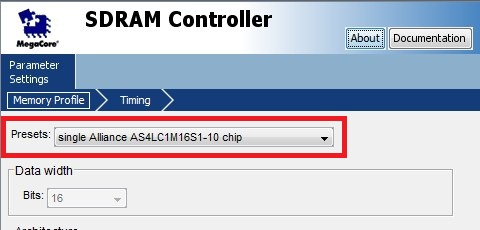
\includegraphics[scale=0.6]{9}
	\caption{SDRAM controller}
	\label{fig:sdram_con}
\end{figure}


\begin{figure}[!h]
	\centering
	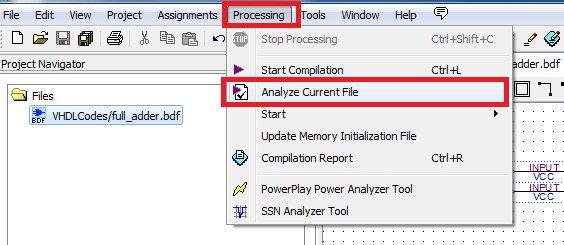
\includegraphics[scale=0.6]{10}
	\caption{SDRAM connections}
	\label{fig:sdram_connections}
\end{figure}


\begin{figure}[!h]
	\centering
	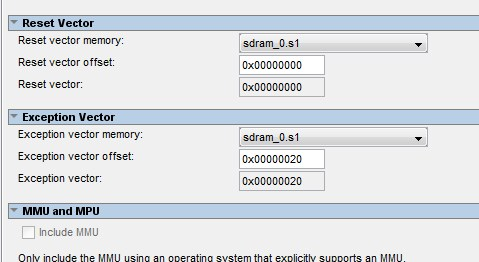
\includegraphics[scale=0.6]{11}
	\caption{Select SDRAM as vector memories}
	\label{fig:sdram_vector_memory}
\end{figure}


Next, we will add `Switches' to control the amplitude of the sine waves. For this add the PIO device of `8 bit with type input', and rename it as `switch', as shown in Fig. \ref{fig:switchForAmplitude} . Finally, go to System$\rightarrow$Assign base addresses, and generate the system. 

\begin{figure}[!h]
	\centering
	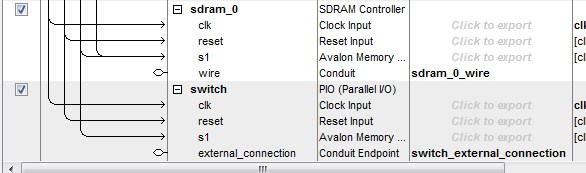
\includegraphics[scale=0.65]{12}
	\caption{Add switches for controlling the amplitude of sine waves}
	\label{fig:switchForAmplitude}
\end{figure}


\subsection{Modify Top level Quartus design}
Now, open the `Uart\_top.bdf' file in Quartus. Right click on the `Uart\_Qsys' block and select `Update symbol or block'; then select the option `Selected symbol(s) or block(s)' and press OK. It will display all the ports for `SDRAM' and switches. Next, we need to assign the correct `pin names' to these ports, as shown in Fig. \ref{fig:SDRAM_Pinassg}.  

\begin{figure}[!h]
	\centering
	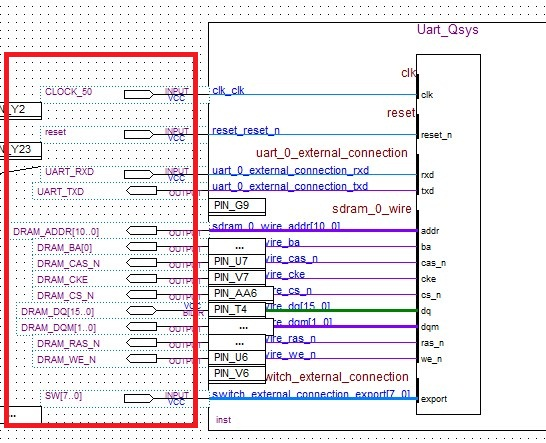
\includegraphics[scale=0.65]{13}
	\caption{Assigning Pins to SDRAM and Switches}
	\label{fig:SDRAM_Pinassg}
\end{figure}

Note that, there should be `-3 ns clock delay' for SDRAM as compare to FPGA clock, therefore we need to add the clock with `-3 ns delay'. For this, double click on the Uart\_top.bdf (anywhere in the file), and select `MegaWizard Plug-In Manager'. Then select `Create a new custom megafunction variation' in the popped-up window and click next. Now, select \textbf{ALTPLL} from \textbf{IO} in \textbf{Installed Plug-Ins} option, as shown in Fig. \ref{fig:dram_clock_altpll}, and click next. Then, follow the figures from Fig. \ref{fig:altpllCreation1} to Fig. \ref{fig:altpllCreation6} to add the ALTPLL to current design i.e. `Uart\_top.bdf'. Finally, connect the ports of this design as shown in Fig. \ref{fig:altpllCreation7}. Note that, in these connections, output of ATLPLL design is connected to `DRAM\_CLK', which is clock-port for DRAM. Lastly, compile and load the design on FPGA board. 

\begin{figure}[!h]
	\centering
	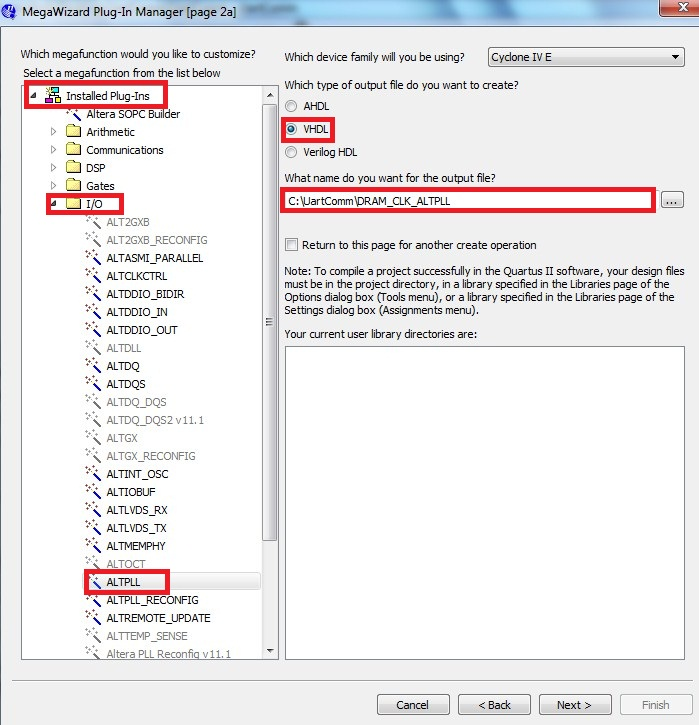
\includegraphics[scale=0.4]{14}
	\caption{ALTPLL generation}
	\label{fig:dram_clock_altpll}
\end{figure}

\begin{figure}[!h]
	\centering
	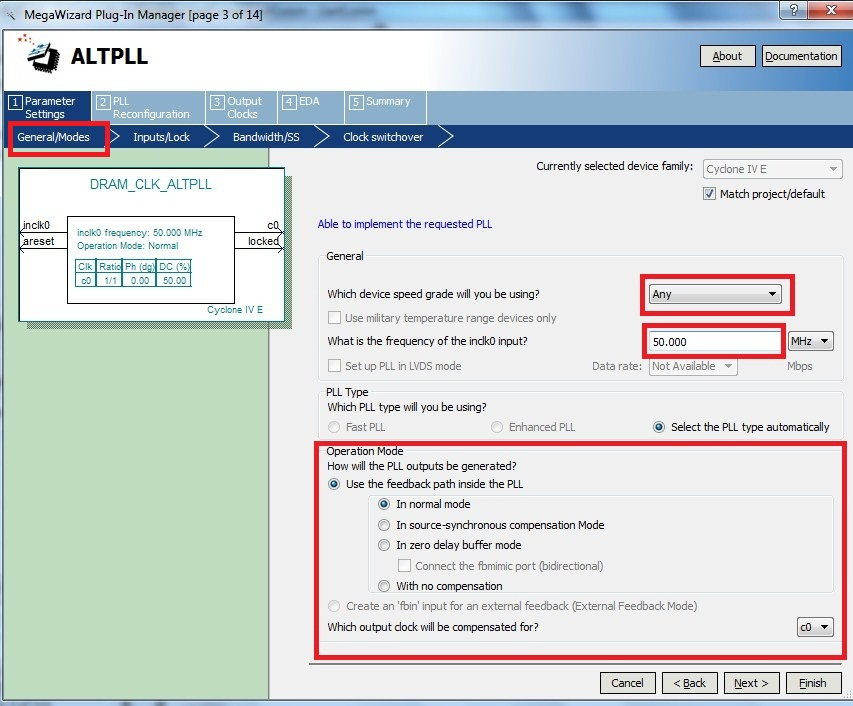
\includegraphics[scale=0.4]{15}
	\caption{ALTPLL creation, step 1}
	\label{fig:altpllCreation1}
\end{figure}

\begin{figure}[!h]
	\centering
	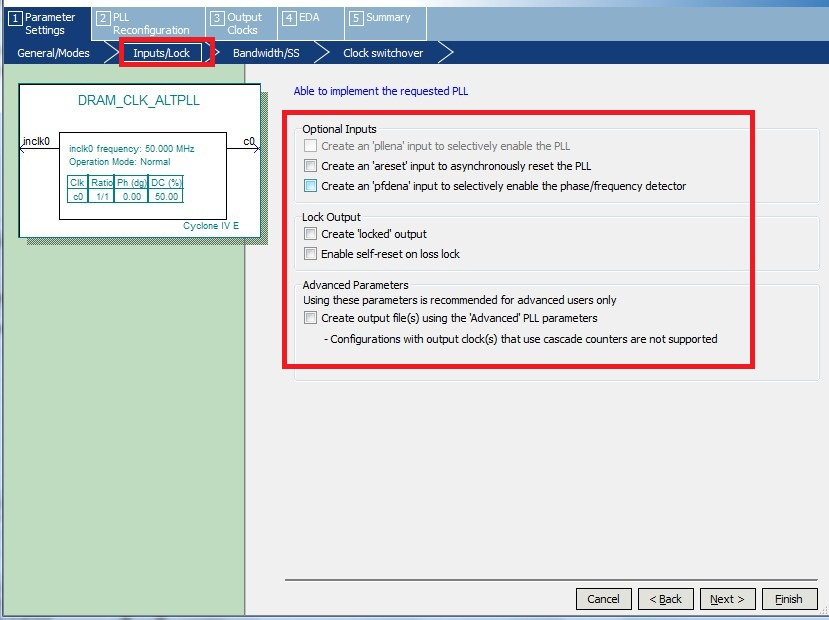
\includegraphics[scale=0.5]{16}
	\caption{ALTPLL creation, step 2}
	\label{fig:altpllCreation2}
\end{figure}

\begin{figure}[!h]
	\centering
	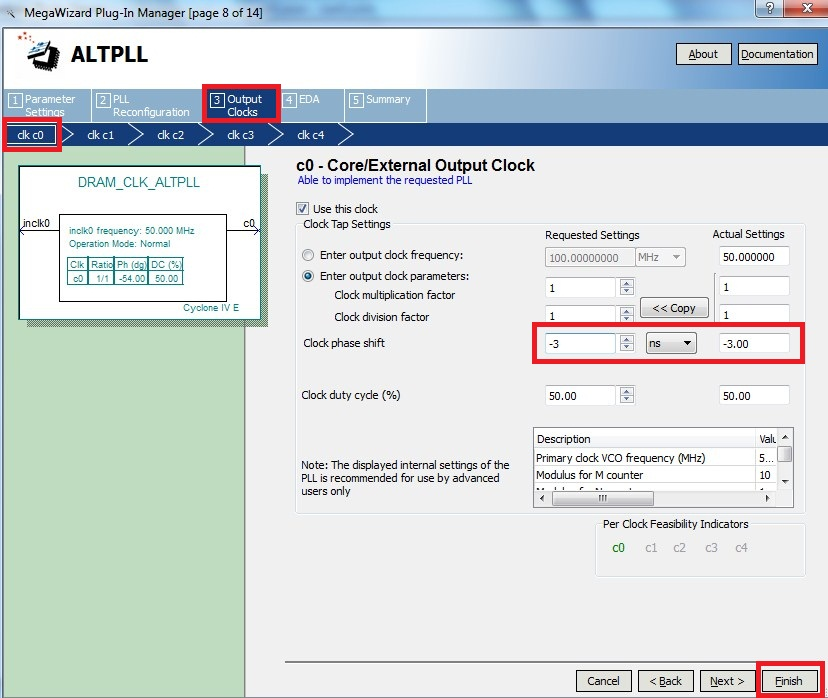
\includegraphics[scale=0.4]{17}
	\caption{ALTPLL creation, step 3}
	\label{fig:altpllCreation3}
\end{figure}

\begin{figure}[!h]
	\centering
	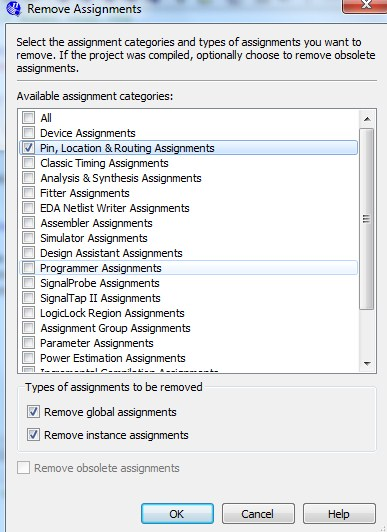
\includegraphics[scale=0.4]{18}
	\caption{ALTPLL creation, step 4}
	\label{fig:altpllCreation4}
\end{figure}

\begin{figure}[!h]
	\centering
	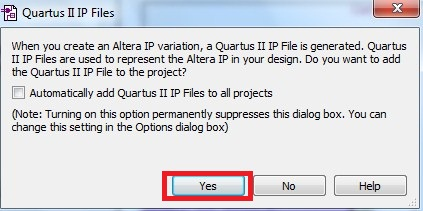
\includegraphics[scale=0.5]{19}
	\caption{ALTPLL creation, step 5}
	\label{fig:altpllCreation5}
\end{figure}

\begin{figure}[!h]
	\centering
	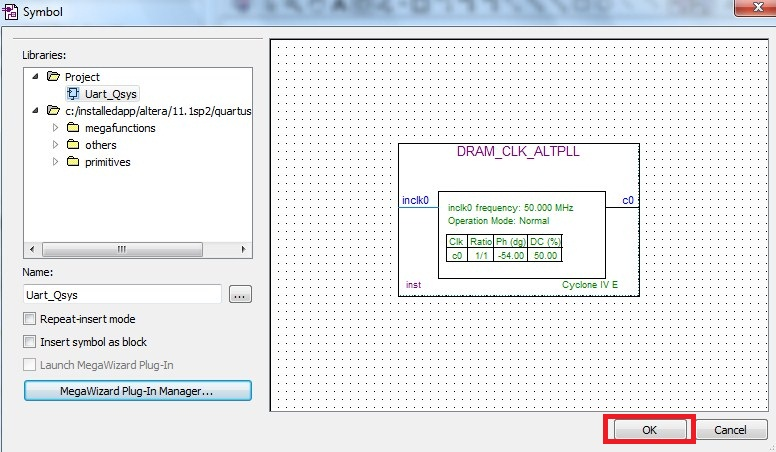
\includegraphics[scale=0.5]{20}
	\caption{ALTPLL creation, step 6}
	\label{fig:altpllCreation6}
\end{figure}

\begin{figure}[!h]
	\centering
	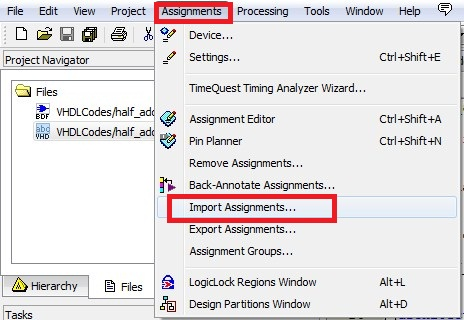
\includegraphics[scale=0.6]{21}
	\caption{Connect ALTPLL design with existing design}
	\label{fig:altpllCreation7}
\end{figure}

\subsection{Updating NIOS design}
Since, we have udpated the QSys design, therefore the corresponding .sopcinfo file is also updated. Further, BSP files depends on the .sopcinfo file, therefore we need to update the BSP as well. For this, right click on `Uart\_comm\_bsp' and go to `NIOS II$\rightarrow$BSP Editor; and update the BSP as shown in Fig. \ref{fig:updateBSPDRAM} and click on `generate' and then click `exit'. Note that, `enable' options are unchecked now, because we are using External memory, which is quite bigger than onchip-memory, so we do not need `small' size options. 

\begin{figure}[!h]
	\centering
	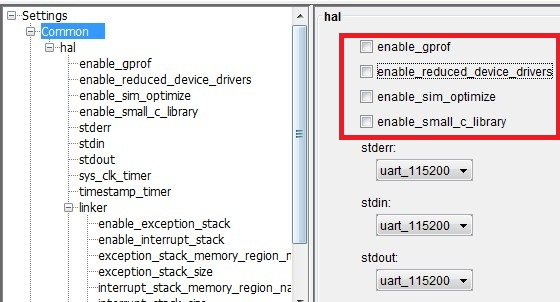
\includegraphics[scale=0.65]{22}
	\caption{Update BSP for new Qsys design}
	\label{fig:updateBSPDRAM}
\end{figure}

Now, update the `hello\_world.c' file as shown in Listing \ref{c:uart_sine_wave}. 

\lstinputlisting[
caption    = {Sin and Cos wave generation},
language = C,
label      = {c:uart_sine_wave}
]{CppCodes/hello_world.c}

In Tera Term, we can save the received values in text file as well. Next, go Files$\rightarrow$Log and select the filename at desired location to save the data e.g. `sineData.txt'. 

Finally, right click on `UART\_comm\_app' in NIOS and go to `Run As$\rightarrow$3 NIOS 2 Hardware'. Now, we can see the decimal values on the screen. If all the switches are at `0' position, then values will be `0.000' as amplitude is zero. Further, we can use any combination of 8 Switches to increase the amplitude of the sine and cosine waves. Also, result will be stored in the  `sineData.txt' file. Content of this file is shown in Fig. \ref{fig:contentLogFile}


\begin{figure}[!h]
	\centering
	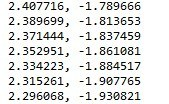
\includegraphics[scale=0.8]{23}
	\caption{Content of `sineData.txt' file}
	\label{fig:contentLogFile}
\end{figure}

\section{Live plotting the data}
In the previous section, we store the sine and cosine wave data on the `sineData.txt' using UART communication. Now, our last task is to plot this data continuously, so that it look line animation. For this save the Listing \ref{pythhon:plotLogData}, in the location where `sineData.txt' is saved. Now, open the command prompt and go to the location of python file. Finally, type \textbf{`python main.py'} and press enter. This will start plotting the waveform continuously based on the data received and stored on the `sineData.txt' file. The corresponding plots are shown in Fig. \ref{fig:plotLogFile}.

\lstinputlisting[
caption    = {Code for live plotting of logged data},
language = Python,
label      = {pythhon:plotLogData}
]{PythonCodes/main.py}

\begin{figure}[!h]
	\centering
	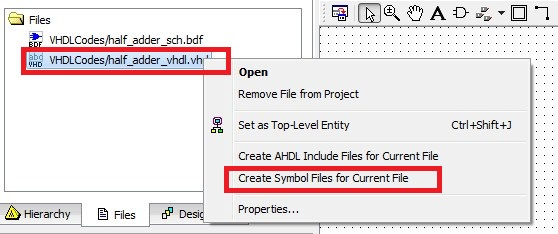
\includegraphics[scale=0.5]{24}
	\caption{Plot of `sineData.txt' file}
	\label{fig:plotLogFile}
\end{figure}


\section{Conclusion}
In this chapter, first we display the `Hello' message using UART and Tera Term. Then, SDRAM is included in the design and correspondingly all the other designs are updated i.e. Quartus and NIOS. Then, the data is stored in the text file and finally it is plotted with the help of Python programming language. 

\section{Introduction}

In previous chapters, we generated the simulation waveforms using modelsim, by providing the input signal values manually; if the number of input signals are very large and/or we have to perform simulation several times, then this process can be quite complex, time consuming and irritating. Suppose input is of 10 bit, and we want to test all the possible values of input i.e. $2^{10}-1$, then it is impossible to do it manually. In such cases, testbenches are very useful; also, tested design more reliable and prefer by the other clients as well. Further, with the help of testbenches, we can generate results in the form of csv (comma separated file), which can be used by other softwares for further analysis e.g. Python, Excel and Matlab etc.  

\textbf{Since testbenches are used for simulation purpose only (not for synthesis), therefore full range of VHDL constructs can be used e.g. keywords `assert', `report' and `for loops' etc. can be used for writing testbenches.}

\textbf{Modelsim-project is created in this chapter for simulations}, which allows the relative path to the files with respect to project directory as shown in Section \ref{sec_read_data_from_file}. Simulation can be run without creating the project, but we need to provide the full path of the files as shown in Lines 30-34 of Listing \ref{vhdl:read_file_ex.vhd}. 

Lastly, mixed modeling is not supported by Altera-Modelsim-starter version, i.e. Verilog designs with VHDL and vice-versa can not be compiled in this version of Modelsim. 

\section{Testbench for combinational circuits}

In this section, various testbenches for combinational circuits are shown, whereas testbenches for sequential circuits are discussed in next section. For simplicity of the codes and better understanding, a simple half adder circuit is tested using various simulation methods. 

\subsection{Half adder}
Listing \ref{vhdl:half_adder.vhd} shows the VHDL code for the half adder which is tested using different ways, 

\lstinputlisting[
language = Vhdl,
caption    = {Half adder},
label      = {vhdl:half_adder.vhd}
]{half_adder.vhd}


\subsection{Simple testbench}

Note that, testbenches are written in separate VHDL files as shown in Listing \ref{vhdl:half_adder_simple_tb.vhd}. Simplest way to write a testbench, is to invoke the `design for testing' in the testbench and provide all the input values in the file,  as explained below, 

\begin{explanation}[Listing \ref{vhdl:half_adder_simple_tb.vhd}]
	In this listing, a testbench with name `half\_adder\_simple\_tb' is defined at Lines 7-8. Note that, entity of testbench is always empty i.e. no ports are defined in the entity (see Lines 7-8). Then 4 signals are defined i.e. a, b, sum and carry (Lines 11-12) inside the architecture body; these signals are then connected to actual half adder design using structural modeling (see Line 15). Lastly, different values are assigned to input signals e.g. `a' and `b' at lines 16 and 17 respectively. 
	
	In Line 22, value of `a' is 0 initially (at 0 ns), then it changes to `1' at 20 ns and again changes to `0' \textbf{at} 40 ns (\textbf{do not confuse with after 40 ns, as after 40 ns is with respect to 0 ns, not with respect to 20 ns}). Similarly, the values of `a' becomes `0' and `1' \textbf{at} 40 and 60 ns respectively. In the same way value of `b' is initially `0' and change to `1' at 40 ns at Line 23. In this way 4 possible combination are generated for two bits (`ab') i.e. 00, 01, 10 and 11 as shown in Fig. \ref{fig:half_adder_simple_tb}; also corresponding outputs, i.e. sum and carry, are shown in the figure. 
	
	\textbf{To generate the waveform, first compile the `half\_adder.vhd and then `half\_adder\_simple\_tb.vhd' (or compile both the file simultaneously.). Then simulate the half\_adder\_simple\_tb.vhd file. Finally, click on `run all' button (which will run the simulation to maximum time i.e. 60 ns here at Line 22)and then click then `zoom full' button (to fit the waveform on the screen), as shown in Fig. \ref{fig:half_adder_simple_tb}.}
\end{explanation}

\textbf{Problem: } Although, the testbench is very simple, but input patterns are not readable. By using the \textbf{process statement} in the testbench, we can make input patterns more readable along with inclusion  of various other features e.g. report generation etc., as shown in next section. 

\lstinputlisting[
language = Vhdl,
caption    = {Simple testbench for half adder},
label      = {vhdl:half_adder_simple_tb.vhd}
]{half_adder_simple_tb.vhd}

\begin{figure}[!h]
	\centering
	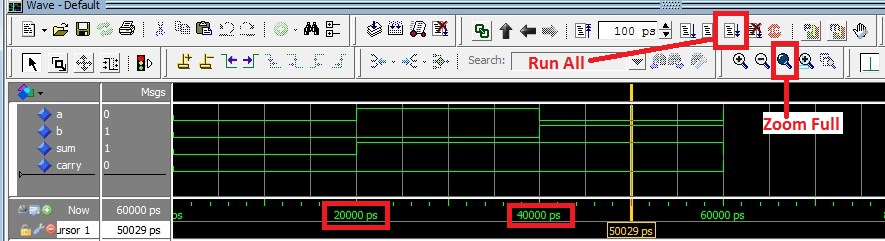
\includegraphics[scale=0.6]{half_adder_simple_tb}
	\caption{Simulation results for Listing \ref{vhdl:half_adder_simple_tb.vhd}}
	\label{fig:half_adder_simple_tb}
\end{figure}


\subsection{Testbench with process statement} \label{sec:tb_with_process_statement}
In Listing \ref{vhdl:half_adder_process_tb.vhd}, process statement is used in the testbench; which includes the input values along with the corresponding output values.  If the specified outputs are not matched with the output generated by half-adder, then errors will be generated. \textbf{Note that, process statement is written without the sensitivity list.}

\begin{explanation}[Listing \ref{vhdl:half_adder_process_tb.vhd}]
	The listing is same as previous listing till Line 15, and then process statement is used to define the input patterns, which can be seen at lines 20-21 (00),  27-28 (01), 33-34 (10) and 39-40 (11). Further, expected outputs are shown below these lines e.g. line 23 shows that the sum is 0 and carry is 0 for input 00; and if the generated output is different from these values, e.g. error is generated by line 50 for input pattern 01 as shown in Fig. \ref{fig:half_adder_process_error_tb}; as sum generated by half\_adder for line 46-47 is 1, whereas expected sum is defined as 0 for this combination at line 49. Note that, the adder output is correct, whereas the expected value is entered incorrectly; and error is displayed on `transcript window' of modelsim. 
	
	Also, `period' is defined as 20 ns at Line 18; and then used after each input values e.g line 22, which indicates that input will be displayed for 20 ns before going to next input values (see in Fig. \ref{fig:half_adder_process_error_tb}).
\end{explanation}

\lstinputlisting[
language = Vhdl,
caption    = {Testbench with process statement},
label      = {vhdl:half_adder_process_tb.vhd}
]{half_adder_process_tb.vhd}

\begin{figure}[!h]
	\centering
	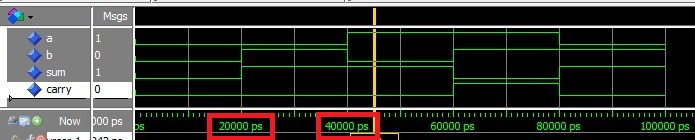
\includegraphics[scale=0.8]{half_adder_process_tb}
	\caption{Simulation results for Listing \ref{vhdl:half_adder_process_tb.vhd}}
	\label{fig:half_adder_process_tb}
\end{figure}

\begin{figure}[!h]
	\centering
	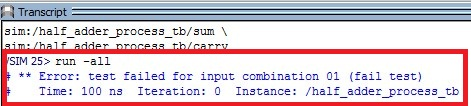
\includegraphics[scale=0.9]{half_adder_process_error_tb}
	\caption{Error generated by Listing \ref{vhdl:half_adder_process_tb.vhd}}
	\label{fig:half_adder_process_error_tb}
\end{figure}

\subsection{Testbench with look-up table}

The inputs patterns can be defined in the form of look-table as well as shown in Listing \ref{vhdl:half_adder_lookup_tb.vhd}, instead of define separately at different location as done in Listing \ref {vhdl:half_adder_process_tb.vhd} e.g. at lines 20 and 27 etc. 

\begin{explanation}[Listing \ref{vhdl:half_adder_lookup_tb.vhd}]
	Basic concept of this Listing is similar to Listing \ref {vhdl:half_adder_process_tb.vhd} but written in different style. Testbench with lookup table can be  written using three steps as shown below, 
	
	\begin{enumerate}
		\item \textbf{Define record : } First we need to define a record which contains the all the possible columns in the look table. Here, there are four possible columns i.e. a, b, sum and carry, which are defined in record at Lines 15-18. 
		
		\item \textbf{Create lookup table : }  Next, we need to define the lookup table values, which is done at Lines 20-28. Here positional method is used for assigning the values to columns (see line 22-27); further, name-association method can also be used as shown in the comment at Line 23. 
		
		\item \textbf{Assign values to signals : } Then the values of the lookup table need to be assigned to half\_adder entity (one by one). For this `for loop' is used at line 35, which assigns the values of ``test-vector's 'a' and 'b' '' to signal `a' and `b' (see comment at Line 36 for better understanding). Similarly, expected values of sum and carry are generated at Lines 41-44. Lastly, report is generated for wrong outputs at Lines 46-50. 
		\\
		\\
		The simulations results and reported-error are shown in Fig. \ref{fig:half_adder_lookup_tb} and Fig. \ref{fig:half_adder_lookup_error_tb} respectively. 
	\end{enumerate}
\end{explanation}

\lstinputlisting[
language = Vhdl,
caption    = {Testbench with look-up table},
label      = {vhdl:half_adder_lookup_tb.vhd}
]{half_adder_lookup_tb.vhd}

\begin{figure}[!h]
	\centering
	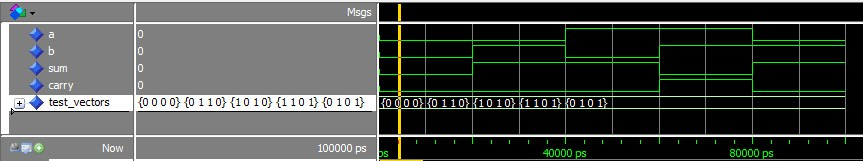
\includegraphics[scale=0.6]{half_adder_lookup_tb}
	\caption{Simulation results for Listing \ref{vhdl:half_adder_lookup_tb.vhd}}
	\label{fig:half_adder_lookup_tb}
\end{figure}

\begin{figure}[!h]
	\centering
	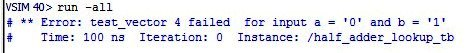
\includegraphics[scale=0.9]{half_adder_lookup_error_tb}
	\caption{Error generated by Listing \ref{vhdl:half_adder_lookup_tb.vhd}}
	\label{fig:half_adder_lookup_error_tb}
\end{figure}

\subsection{Read data from file} \label{sec_read_data_from_file}

In this section, data from file `read\_file\_ex.txt' is read and displayed in simulation results. Date stored in the file is shown in Fig. \ref{fig:read_file_table_ex}. 

\begin{figure}[!h]
	\centering
	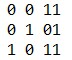
\includegraphics[scale=0.9]{read_file_table_ex}
	\caption{Data in file  `read\_file\_ex.txt'}
	\label{fig:read_file_table_ex}
\end{figure}

\begin{explanation}[Listing \ref{vhdl:read_file_ex.vhd}]
	To read the file, first we need to define a buffer of type `text', which can store the values of the file in it, as shown in Line 17; file is open in read-mode and values are stored in this buffer at Line 32.  
	
	Next, we need to define the variable to read the value from the buffer. Since there are 4 types of values (i.e. a, b, c and spaces) in file `read\_file\_ex.txt', therefore we need to define 4 variables to store them, as shown in Line 24-26. Since, variable c is of 2 bit, therefore Line 25 is 2-bit vector; further, for spaces, variable of character type is defined at Line 26. 
	
	Then, values are read and store in the variables at Lines 36-42. Lastly, these values are assigned to appropriate signals at Lines 45-47. Finally, file is closed at Line 52. The simulation results of the listing are show in Fig. \ref{fig:read_file_ex}. 
\end{explanation}

\lstinputlisting[
language = Vhdl,
caption    = {Read data from file},
label      = {vhdl:read_file_ex.vhd}
]{read_file_ex.vhd}

\begin{figure}[!h]
	\centering
	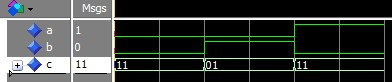
\includegraphics[scale=0.9]{read_file_ex}
	\caption{Simulation results of Listing \ref{vhdl:read_file_ex.vhd} }
	\label{fig:read_file_ex}
\end{figure}


\subsection{Write data to file}\label{sec:writedatafile}

In this part, different types of values are defined in Listing \ref{vhdl:write_file_ex.vhd} and then stored in the file. Here, only `write\_mode' is used for writing the data to file (not the `append\_mode'). 

\begin{explanation}[Listing \ref{vhdl:write_file_ex.vhd}]
	To write the data to the file, first we need to define a buffer, which will load the file on the simulation environment for writing the data during simulation,  as shown in Line 15 (buffer-defined) and Line 27 (load the file to buffer). 
	
	Next, we need to define a variable, which will store the values to write into the buffer, as shown in Line 19. In the listing, this variable stores three types of value i.e. strings (Lines 31 and 34 etc.), signal `a' (Line 35) and variable `b' (Line 37). 
	
	Note that, two keyword are used for writing the data into the file i.e. `write' and `writeline'. `write' keyword store the values in the `write\_col\_to\_output\_buf' and `writeline' writes the values in the file. Remember that, all the `write' statements before the `writeline' will be written in same line e.g. Lines 34-37 will be written in same line as shown in Fig. \ref{fig:write_file_table_ex}. Lastly, the simulation result for the listing is shown in Fig. \ref{fig:write_file_ex}. 
\end{explanation}


\lstinputlisting[
language = Vhdl,
caption    = {Write data to file},
label      = {vhdl:write_file_ex.vhd}
]{write_file_ex.vhd}


\begin{figure}[!h]
	\centering
	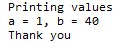
\includegraphics[scale=0.9]{write_file_table_ex}
	\caption{Data in file  `write\_file\_ex.txt'}
	\label{fig:write_file_table_ex}
\end{figure}

\begin{figure}[!h]
	\centering
	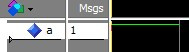
\includegraphics[scale=0.9]{write_file_ex}
	\caption{Simulation results of Listing \ref{vhdl:write_file_ex.vhd} }
	\label{fig:write_file_ex}
\end{figure}


\subsection{Half adder testing using CSV file}
In this section, both read and write operations are performed in Listing \ref{vhdl:read_write_file_ex.vhd}. Further, csv file is used for read and write operations. Content of input and output files are shown in Fig. \ref{fig:half_adder_input} and Fig. \ref{fig:half_adder_output} respectively. 

Please read Listing \ref{vhdl:read_file_ex.vhd} and Listing \ref{vhdl:write_file_ex.vhd} to understand this part, as only these two listings are merged together here. 

\textbf{Addition features added to listing are shown below, }
\begin{enumerate}
	\item Lines 63-64 are added to skip the header row, i.e. any row which does not start with boolean-number(see line 42).
	\item  Also, error will be reported for value `b' if it is not the boolean. Similarly, this functionality can be added to other values as well.
	\item Lastly, errors are reported in CSV file at Lines 96-109. This can be seen in Fig \ref{fig:half_adder_output}. It's always easier to find the location of error using csv file as compare to simulation waveforms (try to find the errors using Fig \ref{fig:half_adder_output} and compare it with Table \ref{fig:half_adder_output}).  
	
\end{enumerate}

\lstinputlisting[
language = Vhdl,
caption    = {Half adder testing using CSV file},
label      = {vhdl:read_write_file_ex.vhd}
]{read_write_file_ex.vhd}


\begin{figure}[!h]
	\centering
	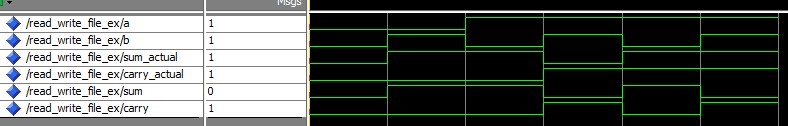
\includegraphics[scale=0.7]{read_write_file_ex}
	\caption{Simulation results of Listing \ref{vhdl:read_write_file_ex.vhd}}
	\label{fig:read_write_file_ex}
\end{figure}

\begin{figure}[!h]
	\centering
	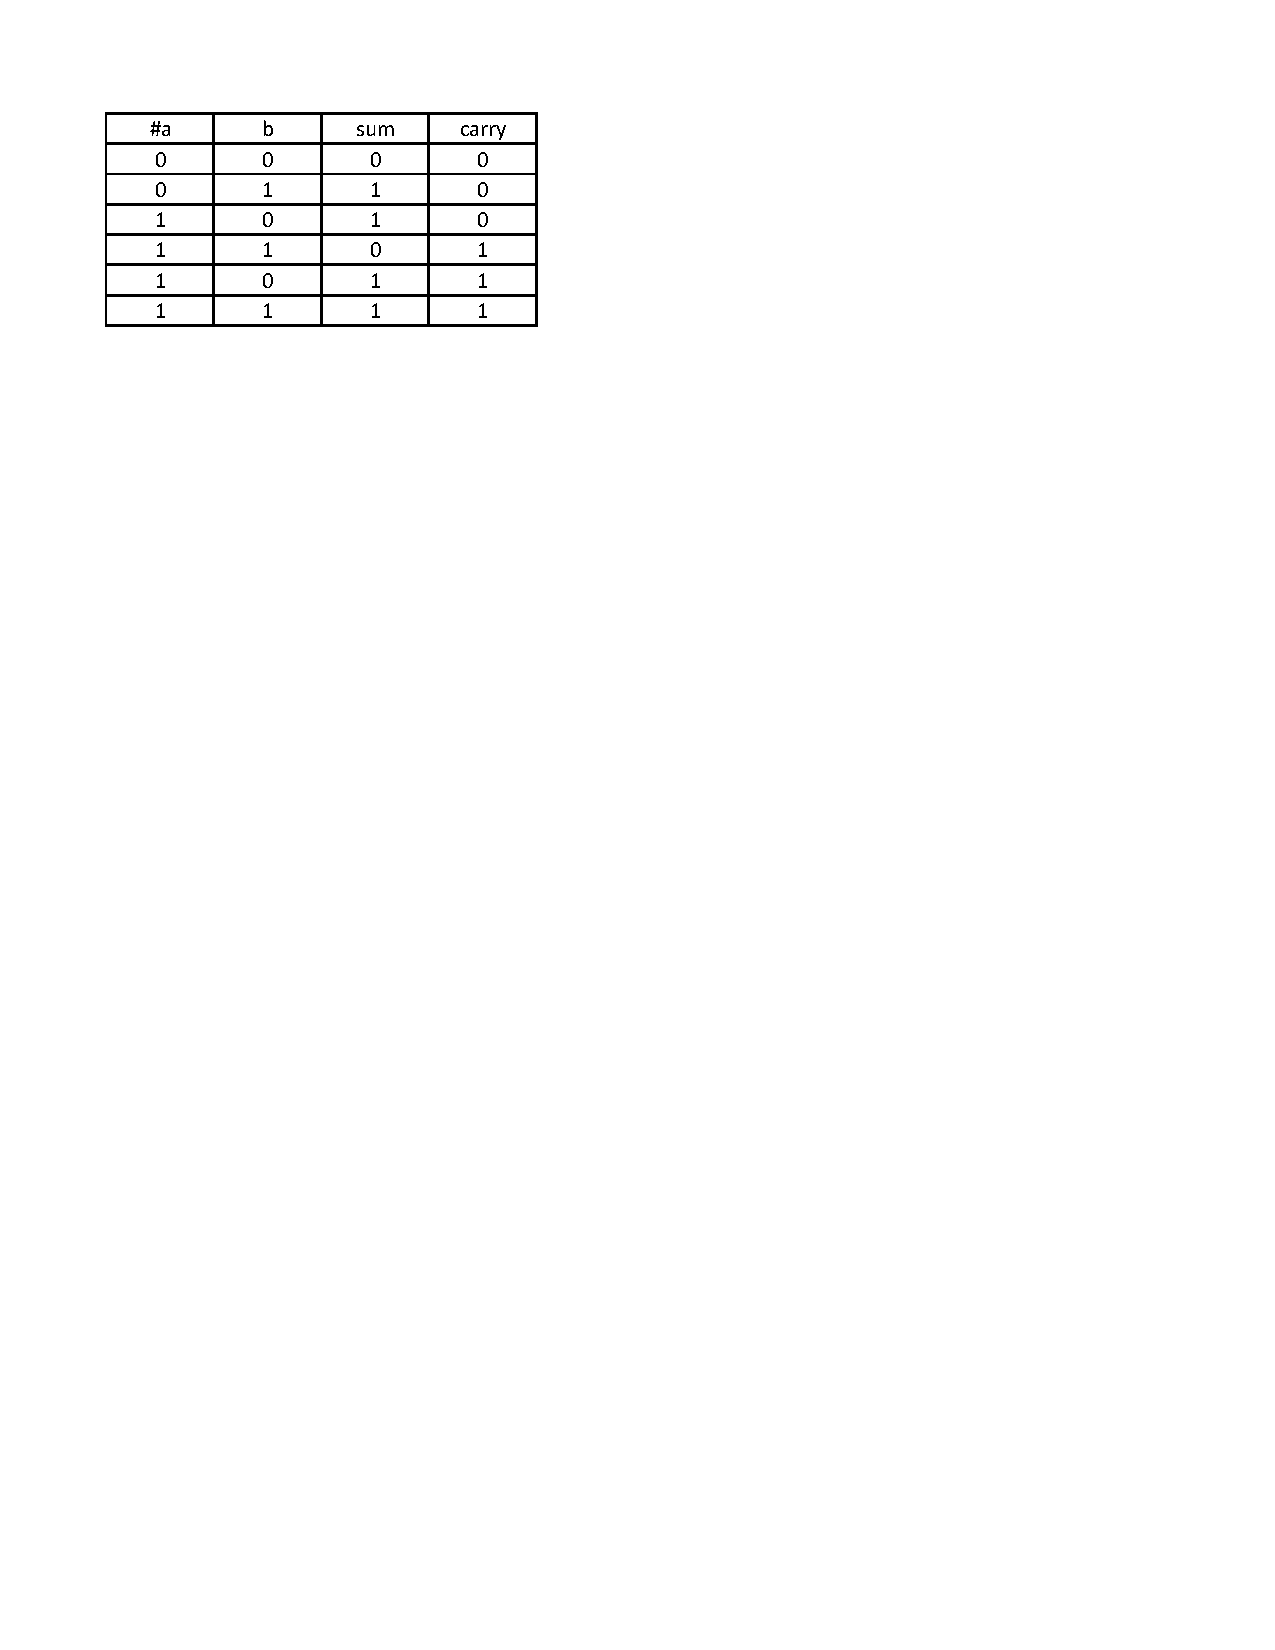
\includegraphics[scale=0.9]{half_adder_input}
	\caption{Content of input file `half\_adder\_input.csv'}
	\label{fig:half_adder_input}
\end{figure}

\begin{figure}[!h]
	\centering
	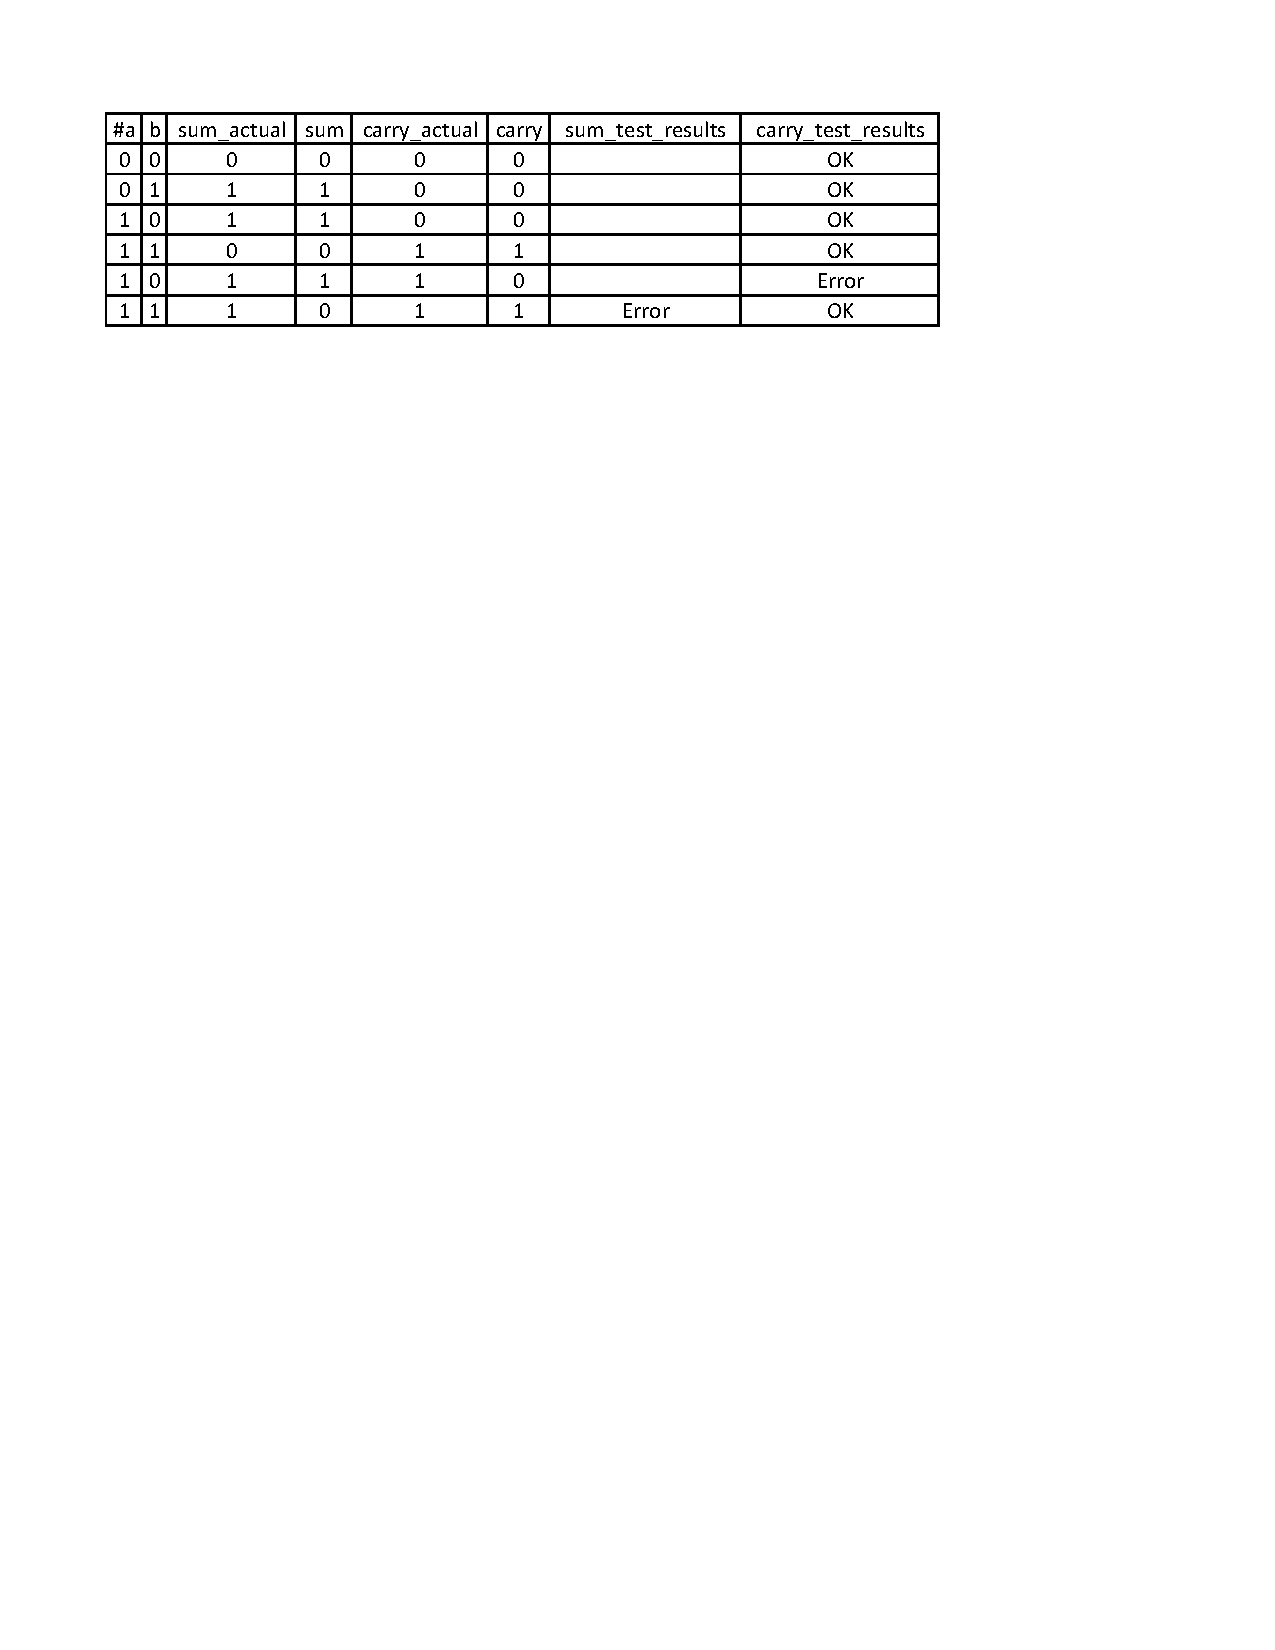
\includegraphics[scale=0.9]{half_adder_output}
	\caption{Content of input file `half\_adder\_output.csv'}
	\label{fig:half_adder_output}
\end{figure}


\section{Testbench for sequential circuits}

In Section \ref{sec:tb_with_process_statement}, we saw the use of process statement for writing the testbench for combination circuits. But, in the case of sequential circuits, we need clock and reset signals; hence two additional blocks are required. Since, clock is generated for complete simulation process, therefore it is defined inside the separate process statement. Whereas, reset signal is required only at the beginning of the operations, hence it is not defined inside the process statement. Rest of the procedures/methods for writing the testbenches for sequential circuits are same as the testbenches of the combinational circuits. 

\subsection{Simulation with infinite duration}
In this section, we have created a testbench which will not stop automatically i.e. if we press the `run all' button then the simulation will run forever, therefore we need to press the `run' button as shown in Fig. \ref{fig:modMCounter_tb}.
\begin{explanation}[Listing \ref{vhdl:modMCounter_tb.vhd}]
	Listing \ref{vhdl:modMCounter_tb.vhd} is the testbench for mod-M counter, which is discussed in Section \ref{sec:ModMCounter}. Here `clk' signal is generated in the separate process block i.e. Lines 27-33; in this way, clock signal will be available throughout the simulation process. Further, reset signal is set to `1' in the beginning and then set to `0' in next clock cycle (Line 37). If there are further, inputs signals, then those signals can be defined in separate process statement, as discussed in combination circuits' testbenches. 
	
	The simulation results are shown in Fig. \ref{fig:modMCounter_tb}, where counter values goes from 0 to 9 as M is set to 10 (i.e. A in hexadecimal). Further, use `run' button for simulating the sequential circuits (instead of run-all), as shown in the figure. 
\end{explanation}


\lstinputlisting[
language = Vhdl,
caption    = {Testbench with infinite duration for modMCounter.vhd},
label      = {vhdl:modMCounter_tb.vhd}
]{modMCounter_tb.vhd}

\begin{figure}[!h]
	\centering
	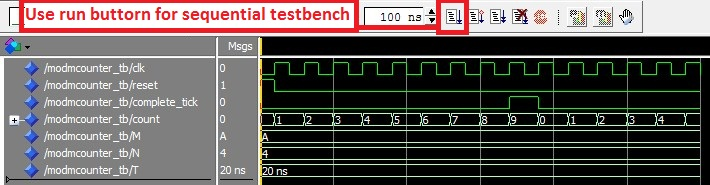
\includegraphics[scale=0.75]{modMCounter_tb}
	\caption{Simulation results of Listing \ref{vhdl:modMCounter_tb.vhd}}
	\label{fig:modMCounter_tb}
\end{figure}

\subsection{Simulation for finite duration and save data}
To run the simulation for the finite duration, we need to provide the `number of clocks' for which we want to run the simulation, as shown in Line 23 of Listing \ref{vhdl:modMCounter_tb2}. Then at Lines 47-52 are added to close the file after desired number of clocks i.e. `num\_of\_clocks'. Also, the data is saved into the file, which is discussed in Section \ref{sec:writedatafile}. Now, if we press the \textbf{run all} button, then the simulator will stop after `num\_of\_clocks' cycles. \textbf{Note that, if the data is in `signed or unsigned' format, then it can not be saved into the file. We need to change the data into other format e.g. `integer', `natural' or `std\_logic\_vector' etc. before saving it into the file, as shown in Line 73}. The simulation waveforms and saved results are shown in Fig. \ref{fig:modMCounter_sim_tb2} and \ref{fig:modMCounter_file_tb2} respectively.

\begin{figure}[!h]
	\centering
	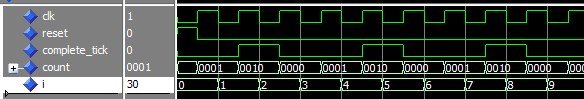
\includegraphics[width=\textwidth]{modMCounter_sim_tb2}
	\caption{Simulation results of Listing \ref{vhdl:modMCounter_tb2}}
	\label{fig:modMCounter_sim_tb2}
\end{figure}

\begin{figure}[!h]
	\centering
	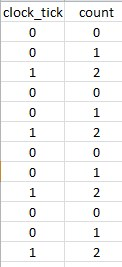
\includegraphics[scale=1]{modMCounter_file_tb2}
	\caption{Partial view of saved data by Listing \ref{vhdl:modMCounter_tb2}}
	\label{fig:modMCounter_file_tb2}
\end{figure}

\lstinputlisting[
language = Vhdl,
caption    = {Testbench with finite duration for modMCounter.vhd},
label      = {vhdl:modMCounter_tb2}
]{modMCounter_tb2.vhd}


\section{Conclusion}
In this chapter, we learn to write testbenches with different styles for combinational circuits. We saw the methods by which inputs can be read from the file and the outputs can be written in the file. Simulation results and expected results are compared and saved in the csv file and displayed as simulation waveforms; which demonstrated that locating the errors in csv files is easier than the simulation waveforms. Further, we saw the simulation of sequential circuits as well, which is slightly different from combination circuits; but all the methods of combinational circuit simulations can be applied to sequential circuits as well. 